%\documentclass[MTRX3700report.tex]{subfiles}
% Lydia
\documentclass{article}
\usepackage{graphicx}
\usepackage{float}
\usepackage{listings}

\begin{document}
	
	\subsection{Module Requirements: Full Auto Mode}
	The Full Auto Mode module consists of all the control for the robot in full auto mode.	In this mode the user has no control over the robot except for stop and start. Once the robot is placed next to the tilt it will start moving in a well defined manner to achieve a set distance away from the tilt. 
	
	This mode makes strong use of the IR Sensors module uses the following functions from it: 
	
	\begin{itemize}
		\item \textbf{IR\textunderscore Calculate} - Calculates distance to tilt and current IR state.
		\item \textbf{Get\textunderscore S\textunderscore IR\textunderscore state} - this function returns the current state of the IR where: error = 0, too close = 1, too far = 3.
	\end{itemize} 
	Refer to IR Sensors module for more information. 
	
	\subsubsection{Functional Requirements}
	%This section describes the functional requirements of Module X – those requirements that must be met if the module (and system) is to function correctly. 
 
	As this module is for a run mode it requires many other modules to be initialized and running before operation. Many of these modules overlap with ones required to use the IR Sensor module. They include:
	
	\begin{itemize}
		\item \textbf{PWM Setup} converts Timer 2 to PWM mode necessary to output PWM for motor operation.
		\item \textbf{Serial Communications} to receive input from controller change mode to Auto and to start and stop the motors.
		\item \textbf{IR Sensors} to utilize the readings from the IR sensor for control. This also includes any functional requirements necessary for the IR sensors module such as the ADC converter setup.
	\end{itemize} 
	
	
	\paragraph{Inputs}
	%Describe each external input, including signal encoding and timing, message encoding and timing, protocols, file formats, protection against input errors, etc, as relevant.
	
	The Full Auto module takes the following inputs from the IR Sensors module:	
	\begin{itemize}
		\item \textbf{IR state} - This is the state of IR system which is a number from 0 to 3, where 0 = error, 1 = too close, 2 = parallel, 3 = too far.
		\item \textbf{newstate} flag - this flag is set whenever the IR sensor changes state (ie. from too far to too close, or from too close to error).
	\end{itemize} 
	
	\paragraph{Process}
	%Describe the internal signal transformations and/or computer processing functionality required within the module, required performance limits, and error tolerances as appropriate.
	In Full Auto mode the jousting robot changes direction whenever the \textit{newstate} flag is set. This change in direction corresponds to the current \textit{IR state} which indicates if the robot is too close to the tilt (1), too far away from the tilt (3), or there is an error with the IR sensor and it is out of range (0).  This leads to three possible movements:
	
	\begin{enumerate}
		\item IR state = ERROR (0). The robot stops moving and remains stationary.
		\item IR state = TOO\textunderscore CLOSE (1). The robot turns at a set speed and angle away from the tilt to the right.
		\item IR state = TOO\textunderscore FAR (3). The robot turns at a set speed and angle away towards the tilt to the left.
	\end{enumerate}
	
	
	\paragraph{Outputs}
	%Describe outputs that must be produced for the module to function correctly, including timing, frequency, protocols, etc as relevant.
	This module outputs a PWM signal to each motor controlling the direction the jousting robot moves.
	
	\paragraph{Timing}
	%Any required timing or latency specifications that must be met.
	The speed at which the robot can change direction is determined on the efficiency of the IR sensor to quickly and accurately measure the current distance away from the tilt. But the rate that the velocity of the motors can be physically changed is affected by the motor hardware itself and any control system for the motors.
	
	
	\subsubsection{Non-Function (Quality of Service) Requirements}
	%Non-functional requirements do not need to be met for the device to have basic function, but are required to provide specific levels of performance or engineering quality.
	\paragraph{Performance}
	%Requirements such as computational loop time, accuracy, etc.
	
	This Full Auto mode can only be run when at very low speeds or it crashes immediately into the tilt. However even at low speed the robot will eventually drive into the tilt and stop. The movement path of the robot in auto mode is shown in the figure below:
	
	 	\begin{figure}[h]
	 		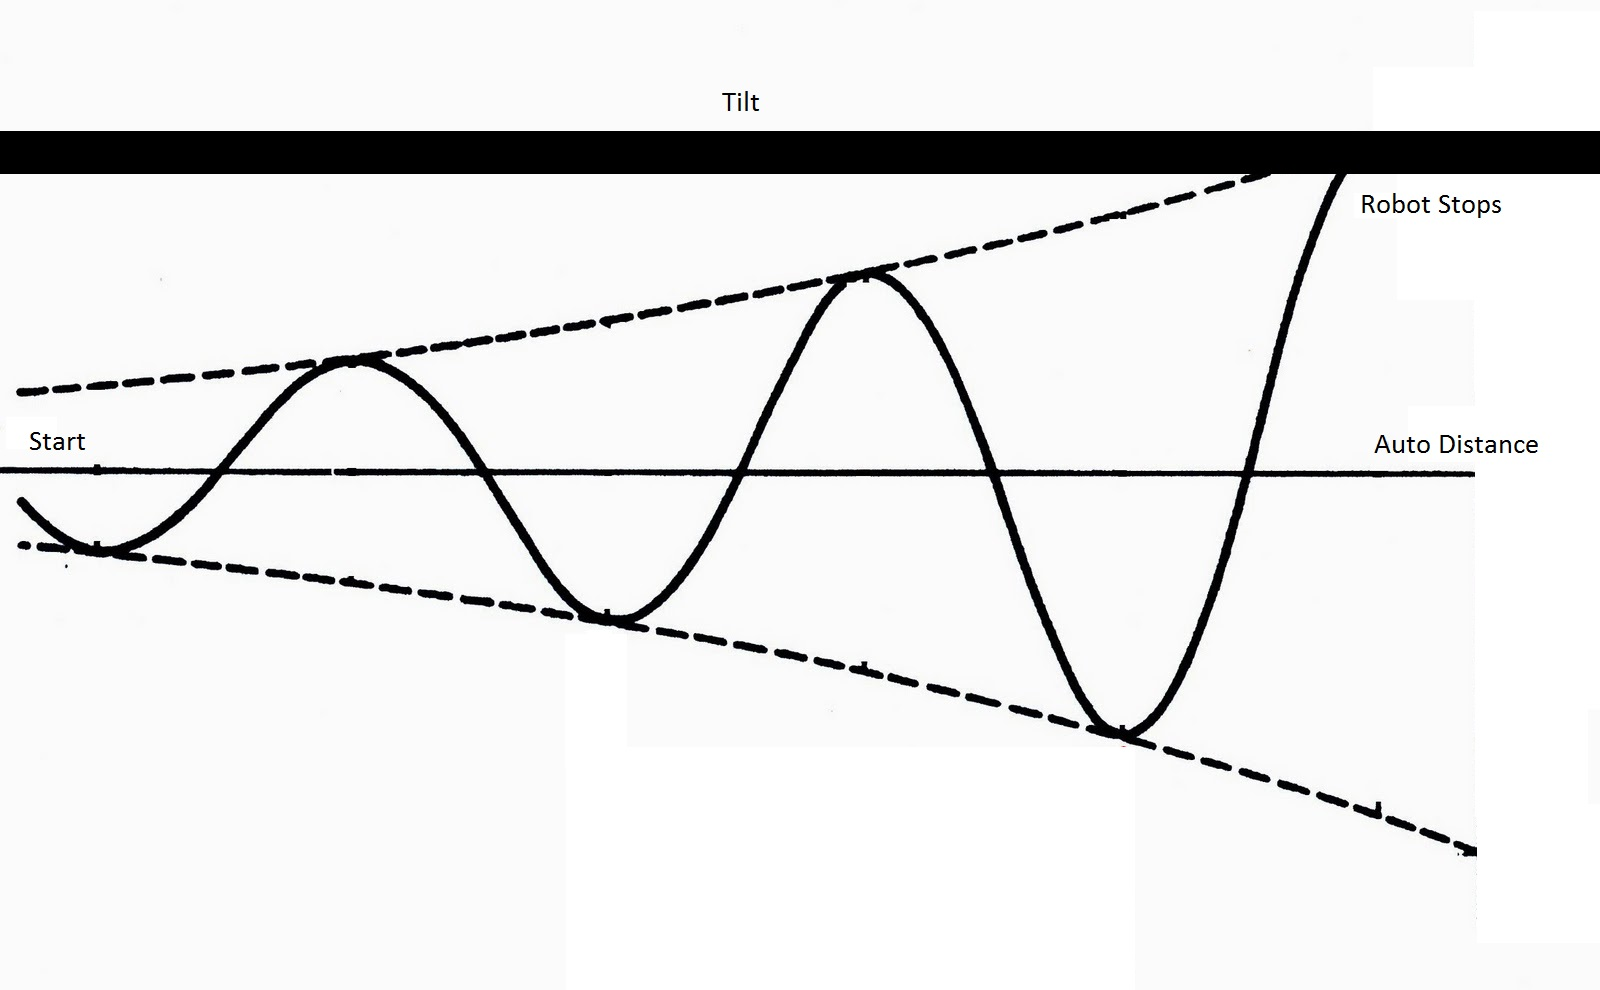
\includegraphics[scale=0.3]{auto_movement.jpg}
	 		\centering
	 		\caption{Full Auto movement path}
	 	\end{figure}
	
	Why this occurs is due to the angle of the IR sensor to the tilt increasing after each turn meaning that it cannot find the correct auto distance until it is too late. However the main reason is thought to be the lack of responsive from the wheels when the \textit{IR state} changes and the robot should turn in the other direction. There is a significant lag whenever the the motors change speed. The cause of this is the lack of feedback control for the motors. 
	
	
	\paragraph{Design Constraints}
	%Practical or commercial considerations, such as programming languages, processor or other 
	As the motor control algorithm dd dot function successfully, there was a need to directly change the speed of the motor for each turn by hard-coding values directly into CCP1 and CCP2 to directly change the PWMs. However without any feedback from the motors this method is extremely unreliable and not very responsive.
	
	
	\subsection{Conceptual Design: Software Module }
		

	\subsubsection{Design Rationale}
	
	The main focus of the Full Auto mode design was to make it simple.
	Without a working control algorithm for the motors it was decided a progressive rate of turning with relation to the distance calculated by the IR sensor would be difficult to implement. Therefore a fixed turn for both directions was implemented with the turning speeds tested by trial and error.
	
	The reason why only one IR sensor was used is also for simplicity. The idea behind this method is that as long as the angle between the tilt and robot does not get too large there is only one distance where the robot is parallel to the tilt. This also requires starting the robot lose to this distance away from the tilt.   
	
	 	 	\begin{figure}[h]
	 	 		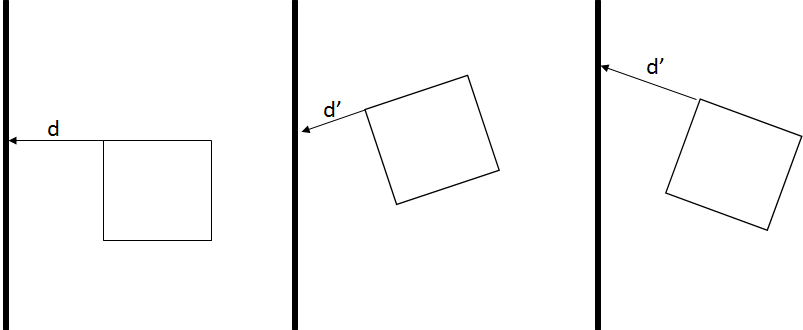
\includegraphics[scale=0.4]{auto_IR.png}
	 	 		\centering
	 	 		\caption{Full Auto IR distance}
	 	 	\end{figure}
	 	 	
	For this method to work effectively the angles of turn must be extremely shallow and the motors must be highly responsive and be able to change speed quickly.

	
	
	\subsubsection{Full Auto Flowchart}

	\begin{figure}[h]
		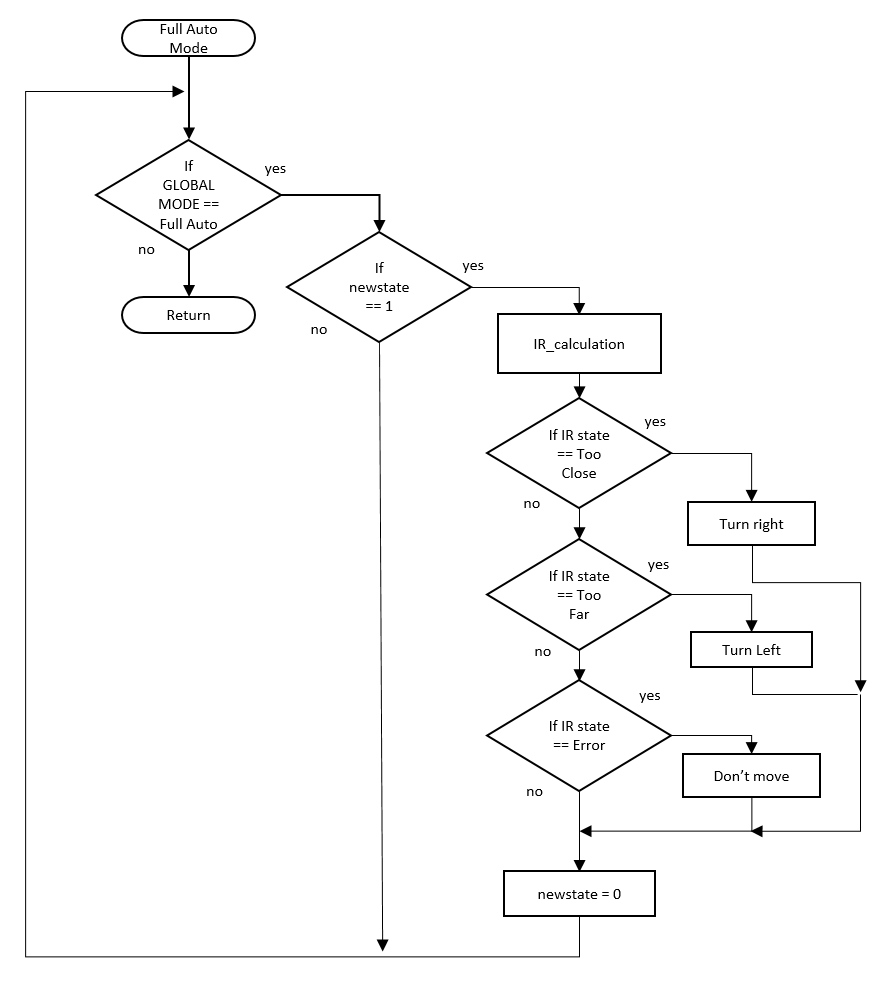
\includegraphics[scale=0.5]{Full_auto_flow.png}
		\centering
		\caption{Full Auto Flowchart}
	\end{figure}
	
	
\end{document}